\documentclass[twoside]{book}

% Packages required by doxygen
\usepackage{fixltx2e}
\usepackage{calc}
\usepackage{doxygen}
\usepackage[export]{adjustbox} % also loads graphicx
\usepackage{graphicx}
\usepackage[utf8]{inputenc}
\usepackage{makeidx}
\usepackage{multicol}
\usepackage{multirow}
\PassOptionsToPackage{warn}{textcomp}
\usepackage{textcomp}
\usepackage[nointegrals]{wasysym}
\usepackage[table]{xcolor}

% Font selection
\usepackage[T1]{fontenc}
\usepackage[scaled=.90]{helvet}
\usepackage{courier}
\usepackage{amssymb}
\usepackage{sectsty}
\renewcommand{\familydefault}{\sfdefault}
\allsectionsfont{%
  \fontseries{bc}\selectfont%
  \color{darkgray}%
}
\renewcommand{\DoxyLabelFont}{%
  \fontseries{bc}\selectfont%
  \color{darkgray}%
}
\newcommand{\+}{\discretionary{\mbox{\scriptsize$\hookleftarrow$}}{}{}}

% Page & text layout
\usepackage{geometry}
\geometry{%
  a4paper,%
  top=2.5cm,%
  bottom=2.5cm,%
  left=2.5cm,%
  right=2.5cm%
}
\tolerance=750
\hfuzz=15pt
\hbadness=750
\setlength{\emergencystretch}{15pt}
\setlength{\parindent}{0cm}
\setlength{\parskip}{3ex plus 2ex minus 2ex}
\makeatletter
\renewcommand{\paragraph}{%
  \@startsection{paragraph}{4}{0ex}{-1.0ex}{1.0ex}{%
    \normalfont\normalsize\bfseries\SS@parafont%
  }%
}
\renewcommand{\subparagraph}{%
  \@startsection{subparagraph}{5}{0ex}{-1.0ex}{1.0ex}{%
    \normalfont\normalsize\bfseries\SS@subparafont%
  }%
}
\makeatother

% Headers & footers
\usepackage{fancyhdr}
\pagestyle{fancyplain}
\fancyhead[LE]{\fancyplain{}{\bfseries\thepage}}
\fancyhead[CE]{\fancyplain{}{}}
\fancyhead[RE]{\fancyplain{}{\bfseries\leftmark}}
\fancyhead[LO]{\fancyplain{}{\bfseries\rightmark}}
\fancyhead[CO]{\fancyplain{}{}}
\fancyhead[RO]{\fancyplain{}{\bfseries\thepage}}
\fancyfoot[LE]{\fancyplain{}{}}
\fancyfoot[CE]{\fancyplain{}{}}
\fancyfoot[RE]{\fancyplain{}{\bfseries\scriptsize Generated by Doxygen }}
\fancyfoot[LO]{\fancyplain{}{\bfseries\scriptsize Generated by Doxygen }}
\fancyfoot[CO]{\fancyplain{}{}}
\fancyfoot[RO]{\fancyplain{}{}}
\renewcommand{\footrulewidth}{0.4pt}
\renewcommand{\chaptermark}[1]{%
  \markboth{#1}{}%
}
\renewcommand{\sectionmark}[1]{%
  \markright{\thesection\ #1}%
}

% Indices & bibliography
\usepackage{natbib}
\usepackage[titles]{tocloft}
\setcounter{tocdepth}{3}
\setcounter{secnumdepth}{5}
\makeindex

% Hyperlinks (required, but should be loaded last)
\usepackage{ifpdf}
\ifpdf
  \usepackage[pdftex,pagebackref=true]{hyperref}
\else
  \usepackage[ps2pdf,pagebackref=true]{hyperref}
\fi
\hypersetup{%
  colorlinks=true,%
  linkcolor=blue,%
  citecolor=blue,%
  unicode%
}

% Custom commands
\newcommand{\clearemptydoublepage}{%
  \newpage{\pagestyle{empty}\cleardoublepage}%
}

\usepackage{caption}
\captionsetup{labelsep=space,justification=centering,font={bf},singlelinecheck=off,skip=4pt,position=top}

%===== C O N T E N T S =====

\begin{document}

% Titlepage & ToC
\hypersetup{pageanchor=false,
             bookmarksnumbered=true,
             pdfencoding=unicode
            }
\pagenumbering{alph}
\begin{titlepage}
\vspace*{7cm}
\begin{center}%
{\Large Tratamento de Poligonos \\[1ex]\large 1.\+0 }\\
\vspace*{1cm}
{\large Generated by Doxygen 1.8.13}\\
\end{center}
\end{titlepage}
\clearemptydoublepage
\pagenumbering{roman}
\tableofcontents
\clearemptydoublepage
\pagenumbering{arabic}
\hypersetup{pageanchor=true}

%--- Begin generated contents ---
\chapter{Projeto de Tratamento de Poligonos referente a disciplina Programação Avançada(dca1202), desenvolvido por Manoel Benedito Neto e Tales Lima Costa}
\label{md__r_e_a_d_m_e}
\Hypertarget{md__r_e_a_d_m_e}
\input{md__r_e_a_d_m_e}
\chapter{Hierarchical Index}
\section{Class Hierarchy}
This inheritance list is sorted roughly, but not completely, alphabetically\+:\begin{DoxyCompactList}
\item \contentsline{section}{Point}{\pageref{class_point}}{}
\item \contentsline{section}{Poligono}{\pageref{class_poligono}}{}
\begin{DoxyCompactList}
\item \contentsline{section}{Retangulo}{\pageref{class_retangulo}}{}
\end{DoxyCompactList}
\end{DoxyCompactList}

\chapter{Class Index}
\section{Class List}
Here are the classes, structs, unions and interfaces with brief descriptions\+:\begin{DoxyCompactList}
\item\contentsline{section}{\hyperlink{classPoint}{Point} }{\pageref{classPoint}}{}
\item\contentsline{section}{\hyperlink{classPoligono}{Poligono} }{\pageref{classPoligono}}{}
\item\contentsline{section}{\hyperlink{classRetangulo}{Retangulo} }{\pageref{classRetangulo}}{}
\end{DoxyCompactList}

\chapter{File Index}
\section{File List}
Here is a list of all files with brief descriptions\+:\begin{DoxyCompactList}
\item\contentsline{section}{\hyperlink{main_8cpp}{main.\+cpp} }{\pageref{main_8cpp}}{}
\item\contentsline{section}{\hyperlink{_point_8cpp}{Point.\+cpp} }{\pageref{_point_8cpp}}{}
\item\contentsline{section}{\hyperlink{_point_8h}{Point.\+h} }{\pageref{_point_8h}}{}
\item\contentsline{section}{\hyperlink{_point__copy_8h}{Point\+\_\+copy.\+h} }{\pageref{_point__copy_8h}}{}
\item\contentsline{section}{\hyperlink{_poligono_8cpp}{Poligono.\+cpp} }{\pageref{_poligono_8cpp}}{}
\item\contentsline{section}{\hyperlink{_poligono_8h}{Poligono.\+h} }{\pageref{_poligono_8h}}{}
\item\contentsline{section}{\hyperlink{_retangulo_8cpp}{Retangulo.\+cpp} }{\pageref{_retangulo_8cpp}}{}
\item\contentsline{section}{\hyperlink{_retangulo_8h}{Retangulo.\+h} }{\pageref{_retangulo_8h}}{}
\end{DoxyCompactList}

\chapter{Class Documentation}
\hypertarget{class_point}{}\section{Point Class Reference}
\label{class_point}\index{Point@{Point}}


A classe {\itshape \hyperlink{class_point}{Point}} define as características e operações que são possíveis realizar com pontos do plano cartesiano.  




{\ttfamily \#include $<$Point.\+h$>$}

\subsection*{Public Member Functions}
\begin{DoxyCompactItemize}
\item 
\hyperlink{class_point_a06c32166c2ad9eac25799ef189b49683}{Point} (float \+\_\+x=0, float \+\_\+y=0)
\begin{DoxyCompactList}\small\item\em {\itshape \hyperlink{class_point}{Point}} é um construtor da classe para atribuir valores as coordenadas x e y, onde, caso não fornecido valores, assume-\/se que x e y recebem o valor de 0. \end{DoxyCompactList}\item 
void \hyperlink{class_point_a428a1676e2fdec6753c42011a1d59d18}{setX} (float \+\_\+x)
\begin{DoxyCompactList}\small\item\em A função {\itshape setX} permite que o usuário possa atribuir valores a variável privada x. \end{DoxyCompactList}\item 
void \hyperlink{class_point_a9868c4601b0ea0c2d0de20fe41ee0e49}{setY} (float \+\_\+y)
\begin{DoxyCompactList}\small\item\em A função {\itshape setY} permite que o usuário possa atribuir valores a variável privada y. \end{DoxyCompactList}\item 
void \hyperlink{class_point_ab5385c6d9bfa841e641e4709fc9f14cc}{set\+XY} (float \+\_\+x, float \+\_\+y)
\begin{DoxyCompactList}\small\item\em Em {\itshape set\+XY}, o usuário tem a disponibilidade de atribuir valores, respectivamente, as variáveis privada x e y. \end{DoxyCompactList}\item 
float \hyperlink{class_point_acc27466778cc87a662bba40268c4c0c8}{getX} ()
\begin{DoxyCompactList}\small\item\em A função {\itshape getX} retorna a coordenada x. \end{DoxyCompactList}\item 
float \hyperlink{class_point_a3cccbca94719ddde353cce86ce0e2f64}{getY} ()
\begin{DoxyCompactList}\small\item\em A função {\itshape getY} retorna a coordenada y. \end{DoxyCompactList}\item 
void \hyperlink{class_point_a6bcf8fd2524ecc4d5b6c1dc942d541a5}{add} (\hyperlink{class_point}{Point} p1)
\begin{DoxyCompactList}\small\item\em É atribuída a função {\itshape add} a utilidade de adicionar às coordenadas (x, y) do ponto os valores das coordenadas de um ponto {\bfseries P1(x1,y1)}. \end{DoxyCompactList}\item 
void \hyperlink{class_point_af7d9e533f0030edf4ab28fdc0f12acd4}{sub} (\hyperlink{class_point}{Point} p1)
\begin{DoxyCompactList}\small\item\em É atribuída a função {\itshape sub} a utilidade de subtrair às coordenadas (x, y) do ponto os valores das coordenadas de um ponto {\bfseries P1(x1,y1)}. \end{DoxyCompactList}\item 
void \hyperlink{class_point_a6233714649b03294a020827fb53eb8ad}{norma} ()
\begin{DoxyCompactList}\small\item\em A função {\itshape norma} calcula a norma de ponto a ponto. \end{DoxyCompactList}\item 
void \hyperlink{class_point_ad9676e36f3444534b609e3c68422239a}{translada} (float a, float b)
\begin{DoxyCompactList}\small\item\em A função {\itshape translada} permite a translação do ponto em (x+a, y+b). \end{DoxyCompactList}\item 
void \hyperlink{class_point_a1fb5c2501c27ab2cbc99d06c2a26a741}{imprime} ()
\begin{DoxyCompactList}\small\item\em A função {\itshape imprime} permite imprimir na tela as coordenadas do ponto na forma (xpos, ypos). \end{DoxyCompactList}\item 
void \hyperlink{class_point_a428a1676e2fdec6753c42011a1d59d18}{setX} (float \+\_\+x)
\item 
void \hyperlink{class_point_a9868c4601b0ea0c2d0de20fe41ee0e49}{setY} (float \+\_\+y)
\item 
void \hyperlink{class_point_ab5385c6d9bfa841e641e4709fc9f14cc}{set\+XY} (float \+\_\+x, float \+\_\+y)
\item 
float \hyperlink{class_point_acc27466778cc87a662bba40268c4c0c8}{getX} ()
\item 
float \hyperlink{class_point_a3cccbca94719ddde353cce86ce0e2f64}{getY} ()
\item 
void \hyperlink{class_point_a6bcf8fd2524ecc4d5b6c1dc942d541a5}{add} (\hyperlink{class_point}{Point} p1)
\item 
void \hyperlink{class_point_af7d9e533f0030edf4ab28fdc0f12acd4}{sub} (\hyperlink{class_point}{Point} p1)
\item 
void \hyperlink{class_point_a6233714649b03294a020827fb53eb8ad}{norma} ()
\item 
void \hyperlink{class_point_ad9676e36f3444534b609e3c68422239a}{translada} (float a, float b)
\item 
void \hyperlink{class_point_a1fb5c2501c27ab2cbc99d06c2a26a741}{imprime} ()
\end{DoxyCompactItemize}


\subsection{Detailed Description}
A classe {\itshape \hyperlink{class_point}{Point}} define as características e operações que são possíveis realizar com pontos do plano cartesiano. 

\subsection{Constructor \& Destructor Documentation}
\mbox{\Hypertarget{class_point_a06c32166c2ad9eac25799ef189b49683}\label{class_point_a06c32166c2ad9eac25799ef189b49683}} 
\index{Point@{Point}!Point@{Point}}
\index{Point@{Point}!Point@{Point}}
\subsubsection{\texorpdfstring{Point()}{Point()}}
{\footnotesize\ttfamily Point\+::\+Point (\begin{DoxyParamCaption}\item[{float}]{\+\_\+x = {\ttfamily 0},  }\item[{float}]{\+\_\+y = {\ttfamily 0} }\end{DoxyParamCaption})}



{\itshape \hyperlink{class_point}{Point}} é um construtor da classe para atribuir valores as coordenadas x e y, onde, caso não fornecido valores, assume-\/se que x e y recebem o valor de 0. 


\begin{DoxyParams}{Parameters}
{\em \+\_\+x} & é a coordenada x do ponto no plano cartesiano. \\
\hline
{\em \+\_\+y} & é a coordenada y do ponto no plano cartesiano. \\
\hline
\end{DoxyParams}

\begin{DoxyCode}
7                               \{
8     x = \_x;
9     y = \_y;
10 \}
\end{DoxyCode}


\subsection{Member Function Documentation}
\mbox{\Hypertarget{class_point_a6bcf8fd2524ecc4d5b6c1dc942d541a5}\label{class_point_a6bcf8fd2524ecc4d5b6c1dc942d541a5}} 
\index{Point@{Point}!add@{add}}
\index{add@{add}!Point@{Point}}
\subsubsection{\texorpdfstring{add()}{add()}\hspace{0.1cm}{\footnotesize\ttfamily [1/2]}}
{\footnotesize\ttfamily void Point\+::add (\begin{DoxyParamCaption}\item[{\hyperlink{class_point}{Point}}]{p1 }\end{DoxyParamCaption})}

\mbox{\Hypertarget{class_point_a6bcf8fd2524ecc4d5b6c1dc942d541a5}\label{class_point_a6bcf8fd2524ecc4d5b6c1dc942d541a5}} 
\index{Point@{Point}!add@{add}}
\index{add@{add}!Point@{Point}}
\subsubsection{\texorpdfstring{add()}{add()}\hspace{0.1cm}{\footnotesize\ttfamily [2/2]}}
{\footnotesize\ttfamily void Point\+::add (\begin{DoxyParamCaption}\item[{\hyperlink{class_point}{Point}}]{p1 }\end{DoxyParamCaption})}



É atribuída a função {\itshape add} a utilidade de adicionar às coordenadas (x, y) do ponto os valores das coordenadas de um ponto {\bfseries P1(x1,y1)}. 


\begin{DoxyParams}{Parameters}
{\em p1} & é um ponto para utilizado para fins de soma de suas coordenadas (x,y) ás coordenadas (x,y) do ponto o qual chama a função. \\
\hline
\end{DoxyParams}

\begin{DoxyCode}
29                        \{
30      x= x+p1.\hyperlink{class_point_acc27466778cc87a662bba40268c4c0c8}{getX}();
31      y= y+p1.\hyperlink{class_point_a3cccbca94719ddde353cce86ce0e2f64}{getY}();
32 \}
\end{DoxyCode}
\mbox{\Hypertarget{class_point_acc27466778cc87a662bba40268c4c0c8}\label{class_point_acc27466778cc87a662bba40268c4c0c8}} 
\index{Point@{Point}!getX@{getX}}
\index{getX@{getX}!Point@{Point}}
\subsubsection{\texorpdfstring{get\+X()}{getX()}\hspace{0.1cm}{\footnotesize\ttfamily [1/2]}}
{\footnotesize\ttfamily float Point\+::getX (\begin{DoxyParamCaption}{ }\end{DoxyParamCaption})}

\mbox{\Hypertarget{class_point_acc27466778cc87a662bba40268c4c0c8}\label{class_point_acc27466778cc87a662bba40268c4c0c8}} 
\index{Point@{Point}!getX@{getX}}
\index{getX@{getX}!Point@{Point}}
\subsubsection{\texorpdfstring{get\+X()}{getX()}\hspace{0.1cm}{\footnotesize\ttfamily [2/2]}}
{\footnotesize\ttfamily float Point\+::getX (\begin{DoxyParamCaption}{ }\end{DoxyParamCaption})}



A função {\itshape getX} retorna a coordenada x. 

\begin{DoxyReturn}{Returns}

\end{DoxyReturn}

\begin{DoxyCode}
23                  \{
24      \textcolor{keywordflow}{return} x;
25 \}
\end{DoxyCode}
\mbox{\Hypertarget{class_point_a3cccbca94719ddde353cce86ce0e2f64}\label{class_point_a3cccbca94719ddde353cce86ce0e2f64}} 
\index{Point@{Point}!getY@{getY}}
\index{getY@{getY}!Point@{Point}}
\subsubsection{\texorpdfstring{get\+Y()}{getY()}\hspace{0.1cm}{\footnotesize\ttfamily [1/2]}}
{\footnotesize\ttfamily float Point\+::getY (\begin{DoxyParamCaption}{ }\end{DoxyParamCaption})}

\mbox{\Hypertarget{class_point_a3cccbca94719ddde353cce86ce0e2f64}\label{class_point_a3cccbca94719ddde353cce86ce0e2f64}} 
\index{Point@{Point}!getY@{getY}}
\index{getY@{getY}!Point@{Point}}
\subsubsection{\texorpdfstring{get\+Y()}{getY()}\hspace{0.1cm}{\footnotesize\ttfamily [2/2]}}
{\footnotesize\ttfamily float Point\+::getY (\begin{DoxyParamCaption}{ }\end{DoxyParamCaption})}



A função {\itshape getY} retorna a coordenada y. 

\begin{DoxyReturn}{Returns}

\end{DoxyReturn}

\begin{DoxyCode}
26                  \{
27      \textcolor{keywordflow}{return} y;
28 \}
\end{DoxyCode}
\mbox{\Hypertarget{class_point_a1fb5c2501c27ab2cbc99d06c2a26a741}\label{class_point_a1fb5c2501c27ab2cbc99d06c2a26a741}} 
\index{Point@{Point}!imprime@{imprime}}
\index{imprime@{imprime}!Point@{Point}}
\subsubsection{\texorpdfstring{imprime()}{imprime()}\hspace{0.1cm}{\footnotesize\ttfamily [1/2]}}
{\footnotesize\ttfamily void Point\+::imprime (\begin{DoxyParamCaption}{ }\end{DoxyParamCaption})}

\mbox{\Hypertarget{class_point_a1fb5c2501c27ab2cbc99d06c2a26a741}\label{class_point_a1fb5c2501c27ab2cbc99d06c2a26a741}} 
\index{Point@{Point}!imprime@{imprime}}
\index{imprime@{imprime}!Point@{Point}}
\subsubsection{\texorpdfstring{imprime()}{imprime()}\hspace{0.1cm}{\footnotesize\ttfamily [2/2]}}
{\footnotesize\ttfamily void Point\+::imprime (\begin{DoxyParamCaption}{ }\end{DoxyParamCaption})}



A função {\itshape imprime} permite imprimir na tela as coordenadas do ponto na forma (xpos, ypos). 


\begin{DoxyCode}
44                    \{
45        cout << \textcolor{stringliteral}{"("} << x << \textcolor{stringliteral}{", "} << y << \textcolor{stringliteral}{")"};
46 \}
\end{DoxyCode}
\mbox{\Hypertarget{class_point_a6233714649b03294a020827fb53eb8ad}\label{class_point_a6233714649b03294a020827fb53eb8ad}} 
\index{Point@{Point}!norma@{norma}}
\index{norma@{norma}!Point@{Point}}
\subsubsection{\texorpdfstring{norma()}{norma()}\hspace{0.1cm}{\footnotesize\ttfamily [1/2]}}
{\footnotesize\ttfamily void Point\+::norma (\begin{DoxyParamCaption}{ }\end{DoxyParamCaption})}

\mbox{\Hypertarget{class_point_a6233714649b03294a020827fb53eb8ad}\label{class_point_a6233714649b03294a020827fb53eb8ad}} 
\index{Point@{Point}!norma@{norma}}
\index{norma@{norma}!Point@{Point}}
\subsubsection{\texorpdfstring{norma()}{norma()}\hspace{0.1cm}{\footnotesize\ttfamily [2/2]}}
{\footnotesize\ttfamily void Point\+::norma (\begin{DoxyParamCaption}{ }\end{DoxyParamCaption})}



A função {\itshape norma} calcula a norma de ponto a ponto. 


\begin{DoxyCode}
37                  \{
38        norm = sqrt(x*x + y*y);
39 \}
\end{DoxyCode}
\mbox{\Hypertarget{class_point_a428a1676e2fdec6753c42011a1d59d18}\label{class_point_a428a1676e2fdec6753c42011a1d59d18}} 
\index{Point@{Point}!setX@{setX}}
\index{setX@{setX}!Point@{Point}}
\subsubsection{\texorpdfstring{set\+X()}{setX()}\hspace{0.1cm}{\footnotesize\ttfamily [1/2]}}
{\footnotesize\ttfamily void Point\+::setX (\begin{DoxyParamCaption}\item[{float}]{\+\_\+x }\end{DoxyParamCaption})}

\mbox{\Hypertarget{class_point_a428a1676e2fdec6753c42011a1d59d18}\label{class_point_a428a1676e2fdec6753c42011a1d59d18}} 
\index{Point@{Point}!setX@{setX}}
\index{setX@{setX}!Point@{Point}}
\subsubsection{\texorpdfstring{set\+X()}{setX()}\hspace{0.1cm}{\footnotesize\ttfamily [2/2]}}
{\footnotesize\ttfamily void Point\+::setX (\begin{DoxyParamCaption}\item[{float}]{\+\_\+x }\end{DoxyParamCaption})}



A função {\itshape setX} permite que o usuário possa atribuir valores a variável privada x. 


\begin{DoxyParams}{Parameters}
{\em \+\_\+x} & é o valor atribuído a variável privada x. \\
\hline
\end{DoxyParams}

\begin{DoxyCode}
12                         \{
13     x= \_x;
14 \}
\end{DoxyCode}
\mbox{\Hypertarget{class_point_ab5385c6d9bfa841e641e4709fc9f14cc}\label{class_point_ab5385c6d9bfa841e641e4709fc9f14cc}} 
\index{Point@{Point}!set\+XY@{set\+XY}}
\index{set\+XY@{set\+XY}!Point@{Point}}
\subsubsection{\texorpdfstring{set\+X\+Y()}{setXY()}\hspace{0.1cm}{\footnotesize\ttfamily [1/2]}}
{\footnotesize\ttfamily void Point\+::set\+XY (\begin{DoxyParamCaption}\item[{float}]{\+\_\+x,  }\item[{float}]{\+\_\+y }\end{DoxyParamCaption})}

\mbox{\Hypertarget{class_point_ab5385c6d9bfa841e641e4709fc9f14cc}\label{class_point_ab5385c6d9bfa841e641e4709fc9f14cc}} 
\index{Point@{Point}!set\+XY@{set\+XY}}
\index{set\+XY@{set\+XY}!Point@{Point}}
\subsubsection{\texorpdfstring{set\+X\+Y()}{setXY()}\hspace{0.1cm}{\footnotesize\ttfamily [2/2]}}
{\footnotesize\ttfamily void Point\+::set\+XY (\begin{DoxyParamCaption}\item[{float}]{\+\_\+x,  }\item[{float}]{\+\_\+y }\end{DoxyParamCaption})}



Em {\itshape set\+XY}, o usuário tem a disponibilidade de atribuir valores, respectivamente, as variáveis privada x e y. 


\begin{DoxyParams}{Parameters}
{\em \+\_\+x} & é o valor atribuído a variável privada x. \\
\hline
{\em \+\_\+y} & é o valor atribuído a variável privada y. \\
\hline
\end{DoxyParams}

\begin{DoxyCode}
19                                    \{
20     \hyperlink{class_point_a428a1676e2fdec6753c42011a1d59d18}{setX}(\_x);
21     \hyperlink{class_point_a9868c4601b0ea0c2d0de20fe41ee0e49}{setY}(\_y);
22 \}
\end{DoxyCode}
\mbox{\Hypertarget{class_point_a9868c4601b0ea0c2d0de20fe41ee0e49}\label{class_point_a9868c4601b0ea0c2d0de20fe41ee0e49}} 
\index{Point@{Point}!setY@{setY}}
\index{setY@{setY}!Point@{Point}}
\subsubsection{\texorpdfstring{set\+Y()}{setY()}\hspace{0.1cm}{\footnotesize\ttfamily [1/2]}}
{\footnotesize\ttfamily void Point\+::setY (\begin{DoxyParamCaption}\item[{float}]{\+\_\+y }\end{DoxyParamCaption})}

\mbox{\Hypertarget{class_point_a9868c4601b0ea0c2d0de20fe41ee0e49}\label{class_point_a9868c4601b0ea0c2d0de20fe41ee0e49}} 
\index{Point@{Point}!setY@{setY}}
\index{setY@{setY}!Point@{Point}}
\subsubsection{\texorpdfstring{set\+Y()}{setY()}\hspace{0.1cm}{\footnotesize\ttfamily [2/2]}}
{\footnotesize\ttfamily void Point\+::setY (\begin{DoxyParamCaption}\item[{float}]{\+\_\+y }\end{DoxyParamCaption})}



A função {\itshape setY} permite que o usuário possa atribuir valores a variável privada y. 


\begin{DoxyParams}{Parameters}
{\em \+\_\+y} & é o valor atribuído a variável privada y. \\
\hline
\end{DoxyParams}

\begin{DoxyCode}
16                         \{
17     y= \_y;
18 \}
\end{DoxyCode}
\mbox{\Hypertarget{class_point_af7d9e533f0030edf4ab28fdc0f12acd4}\label{class_point_af7d9e533f0030edf4ab28fdc0f12acd4}} 
\index{Point@{Point}!sub@{sub}}
\index{sub@{sub}!Point@{Point}}
\subsubsection{\texorpdfstring{sub()}{sub()}\hspace{0.1cm}{\footnotesize\ttfamily [1/2]}}
{\footnotesize\ttfamily void Point\+::sub (\begin{DoxyParamCaption}\item[{\hyperlink{class_point}{Point}}]{p1 }\end{DoxyParamCaption})}

\mbox{\Hypertarget{class_point_af7d9e533f0030edf4ab28fdc0f12acd4}\label{class_point_af7d9e533f0030edf4ab28fdc0f12acd4}} 
\index{Point@{Point}!sub@{sub}}
\index{sub@{sub}!Point@{Point}}
\subsubsection{\texorpdfstring{sub()}{sub()}\hspace{0.1cm}{\footnotesize\ttfamily [2/2]}}
{\footnotesize\ttfamily void Point\+::sub (\begin{DoxyParamCaption}\item[{\hyperlink{class_point}{Point}}]{p1 }\end{DoxyParamCaption})}



É atribuída a função {\itshape sub} a utilidade de subtrair às coordenadas (x, y) do ponto os valores das coordenadas de um ponto {\bfseries P1(x1,y1)}. 


\begin{DoxyParams}{Parameters}
{\em p1} & é um ponto para utilizado para fins de soma de suas coordenadas (x,y) ás coordenadas (x,y) do ponto o qual chama a função. \\
\hline
\end{DoxyParams}

\begin{DoxyCode}
33                        \{
34      x= x-p1.\hyperlink{class_point_acc27466778cc87a662bba40268c4c0c8}{getX}();
35      y= y-p1.\hyperlink{class_point_a3cccbca94719ddde353cce86ce0e2f64}{getY}();
36 \}
\end{DoxyCode}
\mbox{\Hypertarget{class_point_ad9676e36f3444534b609e3c68422239a}\label{class_point_ad9676e36f3444534b609e3c68422239a}} 
\index{Point@{Point}!translada@{translada}}
\index{translada@{translada}!Point@{Point}}
\subsubsection{\texorpdfstring{translada()}{translada()}\hspace{0.1cm}{\footnotesize\ttfamily [1/2]}}
{\footnotesize\ttfamily void Point\+::translada (\begin{DoxyParamCaption}\item[{float}]{a,  }\item[{float}]{b }\end{DoxyParamCaption})}

\mbox{\Hypertarget{class_point_ad9676e36f3444534b609e3c68422239a}\label{class_point_ad9676e36f3444534b609e3c68422239a}} 
\index{Point@{Point}!translada@{translada}}
\index{translada@{translada}!Point@{Point}}
\subsubsection{\texorpdfstring{translada()}{translada()}\hspace{0.1cm}{\footnotesize\ttfamily [2/2]}}
{\footnotesize\ttfamily void Point\+::translada (\begin{DoxyParamCaption}\item[{float}]{a,  }\item[{float}]{b }\end{DoxyParamCaption})}



A função {\itshape translada} permite a translação do ponto em (x+a, y+b). 


\begin{DoxyParams}{Parameters}
{\em a} & e b são os valores que identificam o quanto deve ser transladado o ponto. \\
\hline
\end{DoxyParams}

\begin{DoxyCode}
40                                      \{
41        x= x+a;
42        y= y+b;
43 \}
\end{DoxyCode}


The documentation for this class was generated from the following files\+:\begin{DoxyCompactItemize}
\item 
\hyperlink{_point_8h}{Point.\+h}\item 
\hyperlink{_point__copy_8h}{Point\+\_\+copy.\+h}\item 
\hyperlink{_point_8cpp}{Point.\+cpp}\end{DoxyCompactItemize}

\hypertarget{class_poligono}{}\section{Poligono Class Reference}
\label{class_poligono}\index{Poligono@{Poligono}}


A classe {\itshape \hyperlink{class_poligono}{Poligono}} define a estrutura e funcionalidades de um polígono, contituindo-\/se como um conjunto de pontos que, quando manipulado corretamente, é possível realizar-\/se operações de calculo de área, transladar o polígono ou até mesmo rotacioná-\/lo.  




{\ttfamily \#include $<$Poligono.\+h$>$}

Inheritance diagram for Poligono\+:\begin{figure}[H]
\begin{center}
\leavevmode
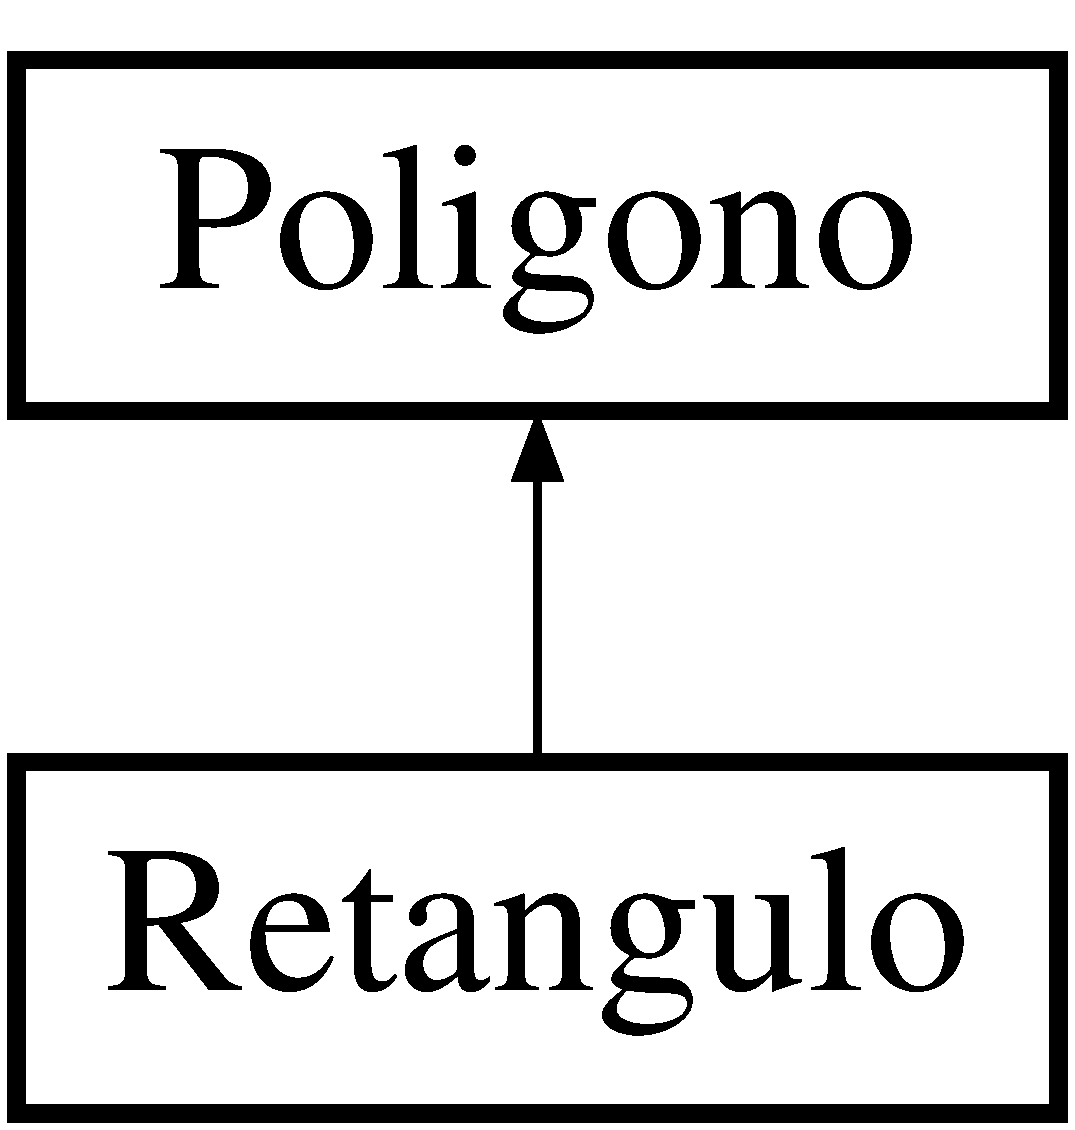
\includegraphics[height=2.000000cm]{class_poligono}
\end{center}
\end{figure}
\subsection*{Public Member Functions}
\begin{DoxyCompactItemize}
\item 
\hyperlink{class_poligono_a9311a9a1496878c09c8508b3636e2870}{Poligono} ()
\item 
void \hyperlink{class_poligono_a4d4cffe97d7190db1f8598b0f9f95763}{setN} (int \+\_\+n)
\begin{DoxyCompactList}\small\item\em Em {\itshape setN} implementa-\/se o número de vertices do polígono. \end{DoxyCompactList}\item 
int \hyperlink{class_poligono_a56257204345b9be3bb5d5fbe45ce63f1}{getN} (void)
\begin{DoxyCompactList}\small\item\em {\itshape getN} retorna a quantidade de vertices do polígono. \end{DoxyCompactList}\item 
void \hyperlink{class_poligono_a0784e2fb0149f6923a42bfabfb073719}{set\+Vertice} (float \+\_\+x, float \+\_\+y)
\begin{DoxyCompactList}\small\item\em {\itshape set\+Vertice} aponta a localização do vertice no plano cartesiano. \end{DoxyCompactList}\item 
float \hyperlink{class_poligono_a051cc49fca5417dbc8c6ba7a1edc2723}{area\+Poligono} (void)
\begin{DoxyCompactList}\small\item\em A função {\itshape area\+Poligono} calcula e retorna a área do poligono prevista a partir do método para encontrar-\/se a \href{https://pt.wikihow.com/Calcular-a-%C3%81rea-de-um-Pol%C3%ADgono}{\tt area de um poligono irregular}. \end{DoxyCompactList}\item 
void \hyperlink{class_poligono_a4d757f52ba9366ab13537fb19b363e1e}{translada\+Poligono} (float a, float b)
\begin{DoxyCompactList}\small\item\em Em {\itshape translada\+Poligono} é possível transladar o polígono para (+a,+b). \end{DoxyCompactList}\item 
void \hyperlink{class_poligono_ad4106abbe48a1c2824da456a4bf4cd71}{rotaciona\+Poligono} (\hyperlink{class_point}{Point} ponto, float theta)
\begin{DoxyCompactList}\small\item\em A função {\itshape rotaciona\+Poligono} rotaciona o polígono em theta graus em relação a um ponto. \end{DoxyCompactList}\item 
void \hyperlink{class_poligono_a87d58f9d4827793eaa811491cce097b0}{imprime\+Poligono} ()
\begin{DoxyCompactList}\small\item\em A função {\itshape imprime\+Poligono} imprime as coordenadas dos pontos que constituem o polígono, distribuídos em ordem anti-\/horária. \end{DoxyCompactList}\end{DoxyCompactItemize}


\subsection{Detailed Description}
A classe {\itshape \hyperlink{class_poligono}{Poligono}} define a estrutura e funcionalidades de um polígono, contituindo-\/se como um conjunto de pontos que, quando manipulado corretamente, é possível realizar-\/se operações de calculo de área, transladar o polígono ou até mesmo rotacioná-\/lo. 

\subsection{Constructor \& Destructor Documentation}
\mbox{\Hypertarget{class_poligono_a9311a9a1496878c09c8508b3636e2870}\label{class_poligono_a9311a9a1496878c09c8508b3636e2870}} 
\index{Poligono@{Poligono}!Poligono@{Poligono}}
\index{Poligono@{Poligono}!Poligono@{Poligono}}
\subsubsection{\texorpdfstring{Poligono()}{Poligono()}}
{\footnotesize\ttfamily Poligono\+::\+Poligono (\begin{DoxyParamCaption}{ }\end{DoxyParamCaption})}


\begin{DoxyCode}
8 \{
9     n = 0;
10 \}
\end{DoxyCode}


\subsection{Member Function Documentation}
\mbox{\Hypertarget{class_poligono_a051cc49fca5417dbc8c6ba7a1edc2723}\label{class_poligono_a051cc49fca5417dbc8c6ba7a1edc2723}} 
\index{Poligono@{Poligono}!area\+Poligono@{area\+Poligono}}
\index{area\+Poligono@{area\+Poligono}!Poligono@{Poligono}}
\subsubsection{\texorpdfstring{area\+Poligono()}{areaPoligono()}}
{\footnotesize\ttfamily float Poligono\+::area\+Poligono (\begin{DoxyParamCaption}\item[{void}]{ }\end{DoxyParamCaption})}



A função {\itshape area\+Poligono} calcula e retorna a área do poligono prevista a partir do método para encontrar-\/se a \href{https://pt.wikihow.com/Calcular-a-%C3%81rea-de-um-Pol%C3%ADgono}{\tt area de um poligono irregular}. 

\begin{DoxyReturn}{Returns}

\end{DoxyReturn}

\begin{DoxyCode}
28                             \{
29     \textcolor{keywordtype}{float} somaPositiva=0, somaNegativa=0;
30     \textcolor{keywordtype}{int} i, j=1;
31     p[n]=p[0];
32     \textcolor{keywordflow}{for}(i=0; i<n; i++)\{
33         somaPositiva+=p[i].\hyperlink{class_point_acc27466778cc87a662bba40268c4c0c8}{getX}()*p[j].\hyperlink{class_point_a3cccbca94719ddde353cce86ce0e2f64}{getY}();
34         j++;
35     \}
36     j=1;
37     \textcolor{keywordflow}{for}(i=0; i<n; i++)\{
38         somaNegativa+=p[j].\hyperlink{class_point_acc27466778cc87a662bba40268c4c0c8}{getX}()*p[i].\hyperlink{class_point_a3cccbca94719ddde353cce86ce0e2f64}{getY}();
39         j++;
40     \}
41     \textcolor{keywordflow}{return} abs(somaPositiva-somaNegativa)/(2.0);
42 \}
\end{DoxyCode}
\mbox{\Hypertarget{class_poligono_a56257204345b9be3bb5d5fbe45ce63f1}\label{class_poligono_a56257204345b9be3bb5d5fbe45ce63f1}} 
\index{Poligono@{Poligono}!getN@{getN}}
\index{getN@{getN}!Poligono@{Poligono}}
\subsubsection{\texorpdfstring{get\+N()}{getN()}}
{\footnotesize\ttfamily int Poligono\+::getN (\begin{DoxyParamCaption}\item[{void}]{ }\end{DoxyParamCaption})}



{\itshape getN} retorna a quantidade de vertices do polígono. 

\begin{DoxyReturn}{Returns}

\end{DoxyReturn}

\begin{DoxyCode}
16                   \{
17     \textcolor{keywordflow}{return} n;
18 \}
\end{DoxyCode}
\mbox{\Hypertarget{class_poligono_a87d58f9d4827793eaa811491cce097b0}\label{class_poligono_a87d58f9d4827793eaa811491cce097b0}} 
\index{Poligono@{Poligono}!imprime\+Poligono@{imprime\+Poligono}}
\index{imprime\+Poligono@{imprime\+Poligono}!Poligono@{Poligono}}
\subsubsection{\texorpdfstring{imprime\+Poligono()}{imprimePoligono()}}
{\footnotesize\ttfamily void Poligono\+::imprime\+Poligono (\begin{DoxyParamCaption}{ }\end{DoxyParamCaption})}



A função {\itshape imprime\+Poligono} imprime as coordenadas dos pontos que constituem o polígono, distribuídos em ordem anti-\/horária. 


\begin{DoxyCode}
91                               \{
92     \textcolor{keywordflow}{for}(\textcolor{keywordtype}{int} i=0; i<(n-1); i++)\{
93         p[i].\hyperlink{class_point_a1fb5c2501c27ab2cbc99d06c2a26a741}{imprime}();
94         cout << \textcolor{stringliteral}{" -> "};
95     \}
96 
97     p[n-1].\hyperlink{class_point_a1fb5c2501c27ab2cbc99d06c2a26a741}{imprime}();
98 \}
\end{DoxyCode}
\mbox{\Hypertarget{class_poligono_ad4106abbe48a1c2824da456a4bf4cd71}\label{class_poligono_ad4106abbe48a1c2824da456a4bf4cd71}} 
\index{Poligono@{Poligono}!rotaciona\+Poligono@{rotaciona\+Poligono}}
\index{rotaciona\+Poligono@{rotaciona\+Poligono}!Poligono@{Poligono}}
\subsubsection{\texorpdfstring{rotaciona\+Poligono()}{rotacionaPoligono()}}
{\footnotesize\ttfamily void Poligono\+::rotaciona\+Poligono (\begin{DoxyParamCaption}\item[{\hyperlink{class_point}{Point}}]{ponto,  }\item[{float}]{theta }\end{DoxyParamCaption})}



A função {\itshape rotaciona\+Poligono} rotaciona o polígono em theta graus em relação a um ponto. 


\begin{DoxyParams}{Parameters}
{\em ponto} & corresponde ao ponto de referência para rotação do polígono. \\
\hline
{\em theta} & é a angulação de rotação desejada em relação ao ponto fornecido. \\
\hline
\end{DoxyParams}

\begin{DoxyCode}
50                                                         \{
51     \textcolor{keywordtype}{double} rad= (theta*M\_PI)/180.;
52     \textcolor{comment}{// transladando o poligono de maneira tal que}
53     \textcolor{comment}{// o ponto fique na origem}
54     \textcolor{keywordflow}{if}(ponto.\hyperlink{class_point_acc27466778cc87a662bba40268c4c0c8}{getX}()<0 && ponto.\hyperlink{class_point_a3cccbca94719ddde353cce86ce0e2f64}{getY}()<0)\{
55         \hyperlink{class_poligono_a4d757f52ba9366ab13537fb19b363e1e}{transladaPoligono}(ponto.\hyperlink{class_point_acc27466778cc87a662bba40268c4c0c8}{getX}(), ponto.\hyperlink{class_point_a3cccbca94719ddde353cce86ce0e2f64}{getY}());
56     \}
57     \textcolor{keywordflow}{else} \textcolor{keywordflow}{if} (ponto.\hyperlink{class_point_acc27466778cc87a662bba40268c4c0c8}{getX}()>0 && ponto.\hyperlink{class_point_a3cccbca94719ddde353cce86ce0e2f64}{getY}()>0)\{
58         \hyperlink{class_poligono_a4d757f52ba9366ab13537fb19b363e1e}{transladaPoligono}(-ponto.\hyperlink{class_point_acc27466778cc87a662bba40268c4c0c8}{getX}(),-ponto.\hyperlink{class_point_a3cccbca94719ddde353cce86ce0e2f64}{getY}());
59     \}
60 
61     \textcolor{keywordflow}{else} \textcolor{keywordflow}{if}( ponto.\hyperlink{class_point_acc27466778cc87a662bba40268c4c0c8}{getX}()<0&& ponto.\hyperlink{class_point_a3cccbca94719ddde353cce86ce0e2f64}{getY}()>0)\{
62         \hyperlink{class_poligono_a4d757f52ba9366ab13537fb19b363e1e}{transladaPoligono}(ponto.\hyperlink{class_point_acc27466778cc87a662bba40268c4c0c8}{getX}(), -ponto.\hyperlink{class_point_a3cccbca94719ddde353cce86ce0e2f64}{getY}());
63     \}
64     \textcolor{keywordflow}{else} \textcolor{keywordflow}{if}( ponto.\hyperlink{class_point_acc27466778cc87a662bba40268c4c0c8}{getX}()>0 && ponto.\hyperlink{class_point_a3cccbca94719ddde353cce86ce0e2f64}{getY}()<0)\{
65         \hyperlink{class_poligono_a4d757f52ba9366ab13537fb19b363e1e}{transladaPoligono}(-ponto.\hyperlink{class_point_acc27466778cc87a662bba40268c4c0c8}{getX}(),ponto.\hyperlink{class_point_a3cccbca94719ddde353cce86ce0e2f64}{getY}());
66     \}
67 
68     \textcolor{comment}{// rotacionando em torno a origem}
69     \textcolor{keywordflow}{for}(\textcolor{keywordtype}{int} i=0; i<=n; i++)\{
70        p[i].\hyperlink{class_point_ab5385c6d9bfa841e641e4709fc9f14cc}{setXY}(  (p[i].getX()*cos(rad)-p[i].getY()*sin(rad)) , (p[i].getX()*sin(rad)+p[i].getY()*
      cos(rad)) );
71     \}
72 
73     \textcolor{comment}{// transladando o poligono de maneira tal que}
74     \textcolor{comment}{// o ponto volte para a sua coordenada inicial}
75     \textcolor{keywordflow}{if}(ponto.\hyperlink{class_point_acc27466778cc87a662bba40268c4c0c8}{getX}()<0 && ponto.\hyperlink{class_point_a3cccbca94719ddde353cce86ce0e2f64}{getY}()<0)\{
76         \hyperlink{class_poligono_a4d757f52ba9366ab13537fb19b363e1e}{transladaPoligono}(-ponto.\hyperlink{class_point_acc27466778cc87a662bba40268c4c0c8}{getX}(), -ponto.\hyperlink{class_point_a3cccbca94719ddde353cce86ce0e2f64}{getY}());
77     \}
78     \textcolor{keywordflow}{else} \textcolor{keywordflow}{if} (ponto.\hyperlink{class_point_acc27466778cc87a662bba40268c4c0c8}{getX}()>0 && ponto.\hyperlink{class_point_a3cccbca94719ddde353cce86ce0e2f64}{getY}()>0)\{
79         \hyperlink{class_poligono_a4d757f52ba9366ab13537fb19b363e1e}{transladaPoligono}(ponto.\hyperlink{class_point_acc27466778cc87a662bba40268c4c0c8}{getX}(),ponto.\hyperlink{class_point_a3cccbca94719ddde353cce86ce0e2f64}{getY}());
80     \}
81 
82     \textcolor{keywordflow}{else} \textcolor{keywordflow}{if}( ponto.\hyperlink{class_point_acc27466778cc87a662bba40268c4c0c8}{getX}()<0&& ponto.\hyperlink{class_point_a3cccbca94719ddde353cce86ce0e2f64}{getY}()>0)\{
83         \hyperlink{class_poligono_a4d757f52ba9366ab13537fb19b363e1e}{transladaPoligono}(-ponto.\hyperlink{class_point_acc27466778cc87a662bba40268c4c0c8}{getX}(), ponto.\hyperlink{class_point_a3cccbca94719ddde353cce86ce0e2f64}{getY}());
84     \}
85     \textcolor{keywordflow}{else} \textcolor{keywordflow}{if}( ponto.\hyperlink{class_point_acc27466778cc87a662bba40268c4c0c8}{getX}()>0 && ponto.\hyperlink{class_point_a3cccbca94719ddde353cce86ce0e2f64}{getY}()<0)\{
86         \hyperlink{class_poligono_a4d757f52ba9366ab13537fb19b363e1e}{transladaPoligono}(ponto.\hyperlink{class_point_acc27466778cc87a662bba40268c4c0c8}{getX}(),-ponto.\hyperlink{class_point_a3cccbca94719ddde353cce86ce0e2f64}{getY}());
87     \}
88 
89 \}
\end{DoxyCode}
\mbox{\Hypertarget{class_poligono_a4d4cffe97d7190db1f8598b0f9f95763}\label{class_poligono_a4d4cffe97d7190db1f8598b0f9f95763}} 
\index{Poligono@{Poligono}!setN@{setN}}
\index{setN@{setN}!Poligono@{Poligono}}
\subsubsection{\texorpdfstring{set\+N()}{setN()}}
{\footnotesize\ttfamily void Poligono\+::setN (\begin{DoxyParamCaption}\item[{int}]{\+\_\+n }\end{DoxyParamCaption})}



Em {\itshape setN} implementa-\/se o número de vertices do polígono. 


\begin{DoxyParams}{Parameters}
{\em \+\_\+n} & corresponde ao número de vertices. \\
\hline
\end{DoxyParams}

\begin{DoxyCode}
13 \{
14     n =\_n;
15 \}
\end{DoxyCode}
\mbox{\Hypertarget{class_poligono_a0784e2fb0149f6923a42bfabfb073719}\label{class_poligono_a0784e2fb0149f6923a42bfabfb073719}} 
\index{Poligono@{Poligono}!set\+Vertice@{set\+Vertice}}
\index{set\+Vertice@{set\+Vertice}!Poligono@{Poligono}}
\subsubsection{\texorpdfstring{set\+Vertice()}{setVertice()}}
{\footnotesize\ttfamily void Poligono\+::set\+Vertice (\begin{DoxyParamCaption}\item[{float}]{\+\_\+x,  }\item[{float}]{\+\_\+y }\end{DoxyParamCaption})}



{\itshape set\+Vertice} aponta a localização do vertice no plano cartesiano. 


\begin{DoxyParams}{Parameters}
{\em \+\_\+x} & é o valor da coordenada x do vertice. \\
\hline
{\em \+\_\+y} & é o valor da coordenada y do vertice. \\
\hline
\end{DoxyParams}

\begin{DoxyCode}
20                                            \{
21     p[n].\hyperlink{class_point_a428a1676e2fdec6753c42011a1d59d18}{setX}(\_x);
22     p[n].\hyperlink{class_point_a9868c4601b0ea0c2d0de20fe41ee0e49}{setY}(\_y);
23     n++;
24 \}
\end{DoxyCode}
\mbox{\Hypertarget{class_poligono_a4d757f52ba9366ab13537fb19b363e1e}\label{class_poligono_a4d757f52ba9366ab13537fb19b363e1e}} 
\index{Poligono@{Poligono}!translada\+Poligono@{translada\+Poligono}}
\index{translada\+Poligono@{translada\+Poligono}!Poligono@{Poligono}}
\subsubsection{\texorpdfstring{translada\+Poligono()}{transladaPoligono()}}
{\footnotesize\ttfamily void Poligono\+::translada\+Poligono (\begin{DoxyParamCaption}\item[{float}]{a,  }\item[{float}]{b }\end{DoxyParamCaption})}



Em {\itshape translada\+Poligono} é possível transladar o polígono para (+a,+b). 


\begin{DoxyParams}{Parameters}
{\em a} & e b são os valores somados a conjutura do polígono para translada-\/lo. \\
\hline
\end{DoxyParams}

\begin{DoxyCode}
44                                                 \{
45     \textcolor{keywordflow}{for}(\textcolor{keywordtype}{int} i=0; i<n; i++)\{
46         p[i].\hyperlink{class_point_ad9676e36f3444534b609e3c68422239a}{translada}(a,b);
47     \}
48 \}
\end{DoxyCode}


The documentation for this class was generated from the following files\+:\begin{DoxyCompactItemize}
\item 
\hyperlink{_poligono_8h}{Poligono.\+h}\item 
\hyperlink{_poligono_8cpp}{Poligono.\+cpp}\end{DoxyCompactItemize}

\hypertarget{class_retangulo}{}\section{Retangulo Class Reference}
\label{class_retangulo}\index{Retangulo@{Retangulo}}


A classe {\itshape \hyperlink{class_retangulo}{Retangulo}} define como é constituído um retângulo qualquer e suas características, que como um polígono, tem estrutura e funcionalidades similares a classe {\itshape \hyperlink{class_poligono}{Poligono}}, herdando-\/a.  




{\ttfamily \#include $<$Retangulo.\+h$>$}

Inheritance diagram for Retangulo\+:\begin{figure}[H]
\begin{center}
\leavevmode
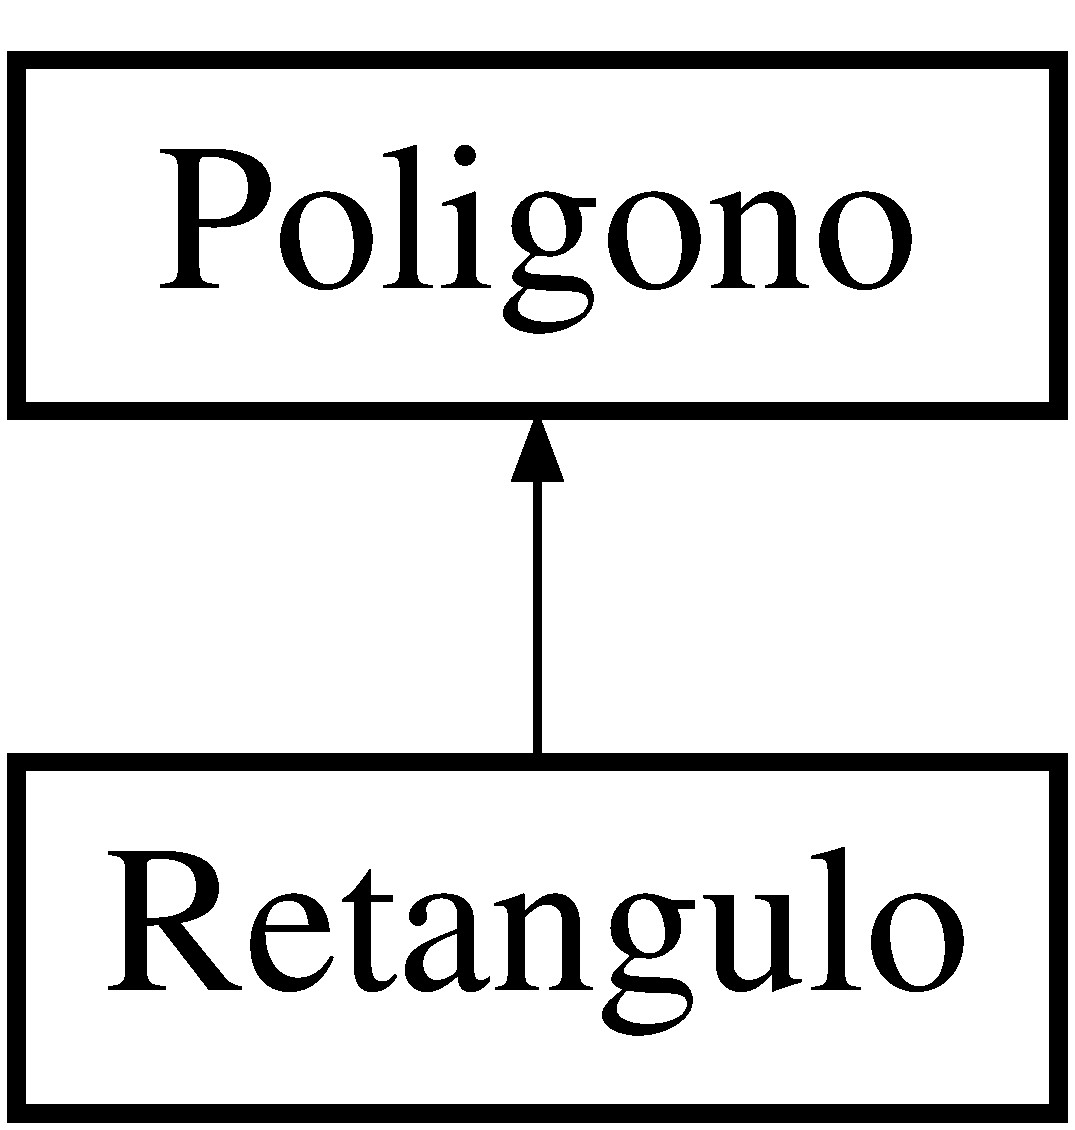
\includegraphics[height=2.000000cm]{class_retangulo}
\end{center}
\end{figure}
\subsection*{Public Member Functions}
\begin{DoxyCompactItemize}
\item 
\hyperlink{class_retangulo_aa2b4dbc14d20e086d8577194af97ef86}{Retangulo} (float \+\_\+xr, float \+\_\+yr, float \+\_\+largura, float \+\_\+altura)
\begin{DoxyCompactList}\small\item\em {\itshape \hyperlink{class_retangulo}{Retangulo}} é uma função construtora para determinar os valores iniciais das características que qualificam o polígono Retângulo. \end{DoxyCompactList}\end{DoxyCompactItemize}


\subsection{Detailed Description}
A classe {\itshape \hyperlink{class_retangulo}{Retangulo}} define como é constituído um retângulo qualquer e suas características, que como um polígono, tem estrutura e funcionalidades similares a classe {\itshape \hyperlink{class_poligono}{Poligono}}, herdando-\/a. 

\subsection{Constructor \& Destructor Documentation}
\mbox{\Hypertarget{class_retangulo_aa2b4dbc14d20e086d8577194af97ef86}\label{class_retangulo_aa2b4dbc14d20e086d8577194af97ef86}} 
\index{Retangulo@{Retangulo}!Retangulo@{Retangulo}}
\index{Retangulo@{Retangulo}!Retangulo@{Retangulo}}
\subsubsection{\texorpdfstring{Retangulo()}{Retangulo()}}
{\footnotesize\ttfamily Retangulo\+::\+Retangulo (\begin{DoxyParamCaption}\item[{float}]{\+\_\+xr,  }\item[{float}]{\+\_\+yr,  }\item[{float}]{\+\_\+largura,  }\item[{float}]{\+\_\+altura }\end{DoxyParamCaption})}



{\itshape \hyperlink{class_retangulo}{Retangulo}} é uma função construtora para determinar os valores iniciais das características que qualificam o polígono Retângulo. 


\begin{DoxyParams}{Parameters}
{\em \+\_\+xr} & é a variável de valor corresponde a coordenada x do ponto superior esquerdo do Retângulo. \\
\hline
{\em \+\_\+yr} & é a variável de valor corresponde a coordenada y do ponto superior esquerdo do Retângulo. \\
\hline
{\em \+\_\+largura} & é o valor da largura do Retângulo. \\
\hline
{\em \+\_\+altura} & é o valor da altura do Retângulo. \\
\hline
\end{DoxyParams}

\begin{DoxyCode}
7 \{
8     xr = \_xr;
9     yr = \_yr;
10     largura = \_largura;
11     altura = \_altura;
12     \hyperlink{class_poligono_a0784e2fb0149f6923a42bfabfb073719}{Poligono::setVertice}(\_xr,\_yr);
13     \hyperlink{class_poligono_a0784e2fb0149f6923a42bfabfb073719}{Poligono::setVertice}(\_xr,\_yr-\_altura);
14     \hyperlink{class_poligono_a0784e2fb0149f6923a42bfabfb073719}{Poligono::setVertice}(\_xr+\_largura,\_yr-\_altura);
15     \hyperlink{class_poligono_a0784e2fb0149f6923a42bfabfb073719}{Poligono::setVertice}(\_xr+\_largura,\_yr);
16 \}
\end{DoxyCode}


The documentation for this class was generated from the following files\+:\begin{DoxyCompactItemize}
\item 
\hyperlink{_retangulo_8h}{Retangulo.\+h}\item 
\hyperlink{_retangulo_8cpp}{Retangulo.\+cpp}\end{DoxyCompactItemize}

\chapter{File Documentation}
\hypertarget{main_8cpp}{}\section{main.\+cpp File Reference}
\label{main_8cpp}\index{main.\+cpp@{main.\+cpp}}
{\ttfamily \#include $<$iostream$>$}\newline
{\ttfamily \#include \char`\"{}Point.\+h\char`\"{}}\newline
{\ttfamily \#include \char`\"{}Poligono.\+h\char`\"{}}\newline
{\ttfamily \#include \char`\"{}Retangulo.\+h\char`\"{}}\newline
\subsection*{Functions}
\begin{DoxyCompactItemize}
\item 
int \hyperlink{main_8cpp_ae66f6b31b5ad750f1fe042a706a4e3d4}{main} ()
\end{DoxyCompactItemize}


\subsection{Function Documentation}
\mbox{\Hypertarget{main_8cpp_ae66f6b31b5ad750f1fe042a706a4e3d4}\label{main_8cpp_ae66f6b31b5ad750f1fe042a706a4e3d4}} 
\index{main.\+cpp@{main.\+cpp}!main@{main}}
\index{main@{main}!main.\+cpp@{main.\+cpp}}
\subsubsection{\texorpdfstring{main()}{main()}}
{\footnotesize\ttfamily int main (\begin{DoxyParamCaption}{ }\end{DoxyParamCaption})}


\begin{DoxyCode}
9 \{
10     \hyperlink{class_retangulo}{Retangulo} R(0,0,3,4);
11     R.imprimePoligono();
12     cout << \textcolor{stringliteral}{"\(\backslash\)n"};
13     cout << R.areaPoligono() << \textcolor{stringliteral}{"\(\backslash\)n"};
14     R.transladaPoligono(-3,4);
15     R.imprimePoligono();
16     cout << \textcolor{stringliteral}{"\(\backslash\)n"} << R.areaPoligono() << \textcolor{stringliteral}{"\(\backslash\)n"};
17 
18     \textcolor{comment}{// centro de massa do retangulo}
19     \hyperlink{class_point}{Point} P;
20     P.\hyperlink{class_point_ab5385c6d9bfa841e641e4709fc9f14cc}{setXY}(-3/2,2);
21     R.rotacionaPoligono(P, 30);
22     R.imprimePoligono();
23     cout << endl << R.areaPoligono() << endl;
24     \textcolor{keywordflow}{return} 0;
25 \}
\end{DoxyCode}

\hypertarget{_point_8cpp}{}\section{Point.\+cpp File Reference}
\label{_point_8cpp}\index{Point.\+cpp@{Point.\+cpp}}
{\ttfamily \#include $<$iostream$>$}\newline
{\ttfamily \#include $<$cmath$>$}\newline
{\ttfamily \#include \char`\"{}Point.\+h\char`\"{}}\newline

\hypertarget{_point_8h}{}\section{Point.\+h File Reference}
\label{_point_8h}\index{Point.\+h@{Point.\+h}}
{\ttfamily \#include $<$iostream$>$}\newline
\subsection*{Classes}
\begin{DoxyCompactItemize}
\item 
class \hyperlink{class_point}{Point}
\begin{DoxyCompactList}\small\item\em A classe {\itshape \hyperlink{class_point}{Point}} define as características e operações que são possíveis realizar com pontos do plano cartesiano. \end{DoxyCompactList}\end{DoxyCompactItemize}

\hypertarget{_point__copy_8h}{}\section{Point\+\_\+copy.\+h File Reference}
\label{_point__copy_8h}\index{Point\+\_\+copy.\+h@{Point\+\_\+copy.\+h}}
{\ttfamily \#include $<$iostream$>$}\newline
{\ttfamily \#include \char`\"{}Point.\+h\char`\"{}}\newline
\subsection*{Classes}
\begin{DoxyCompactItemize}
\item 
class \hyperlink{class_point}{Point}
\begin{DoxyCompactList}\small\item\em A classe {\itshape \hyperlink{class_point}{Point}} define as características e operações que são possíveis realizar com pontos do plano cartesiano. \end{DoxyCompactList}\end{DoxyCompactItemize}

\hypertarget{_poligono_8cpp}{}\section{Poligono.\+cpp File Reference}
\label{_poligono_8cpp}\index{Poligono.\+cpp@{Poligono.\+cpp}}
{\ttfamily \#include $<$iostream$>$}\newline
{\ttfamily \#include $<$cmath$>$}\newline
{\ttfamily \#include \char`\"{}Poligono.\+h\char`\"{}}\newline

\hypertarget{_poligono_8h}{}\section{Poligono.\+h File Reference}
\label{_poligono_8h}\index{Poligono.\+h@{Poligono.\+h}}
{\ttfamily \#include $<$iostream$>$}\newline
{\ttfamily \#include \char`\"{}Point.\+h\char`\"{}}\newline
\subsection*{Classes}
\begin{DoxyCompactItemize}
\item 
class \hyperlink{class_poligono}{Poligono}
\begin{DoxyCompactList}\small\item\em A classe {\itshape \hyperlink{class_poligono}{Poligono}} define a estrutura e funcionalidades de um polígono, contituindo-\/se como um conjunto de pontos que, quando manipulado corretamente, é possível realizar-\/se operações de calculo de área, transladar o polígono ou até mesmo rotacioná-\/lo. \end{DoxyCompactList}\end{DoxyCompactItemize}

\hypertarget{_r_e_a_d_m_e_8md}{}\section{R\+E\+A\+D\+M\+E.\+md File Reference}
\label{_r_e_a_d_m_e_8md}\index{R\+E\+A\+D\+M\+E.\+md@{R\+E\+A\+D\+M\+E.\+md}}

\hypertarget{_retangulo_8cpp}{}\section{Retangulo.\+cpp File Reference}
\label{_retangulo_8cpp}\index{Retangulo.\+cpp@{Retangulo.\+cpp}}
{\ttfamily \#include $<$iostream$>$}\newline
{\ttfamily \#include \char`\"{}Retangulo.\+h\char`\"{}}\newline

\hypertarget{_retangulo_8h}{}\section{Retangulo.\+h File Reference}
\label{_retangulo_8h}\index{Retangulo.\+h@{Retangulo.\+h}}
{\ttfamily \#include $<$iostream$>$}\newline
{\ttfamily \#include \char`\"{}Poligono.\+h\char`\"{}}\newline
\subsection*{Classes}
\begin{DoxyCompactItemize}
\item 
class \hyperlink{class_retangulo}{Retangulo}
\begin{DoxyCompactList}\small\item\em A classe {\itshape \hyperlink{class_retangulo}{Retangulo}} define como é constituído um retângulo qualquer e suas características, que como um polígono, tem estrutura e funcionalidades similares a classe {\itshape \hyperlink{class_poligono}{Poligono}}, herdando-\/a. \end{DoxyCompactList}\end{DoxyCompactItemize}

%--- End generated contents ---

% Index
\backmatter
\newpage
\phantomsection
\clearemptydoublepage
\addcontentsline{toc}{chapter}{Index}
\printindex

\end{document}
